\chapter{Results and summary}
\graphicspath{{Chapter5/Figs/}{Chapter5/Figs/}}

This chapter presents the concrete final results, a concise summary of the project in the form of key aspects of a N/CI and an example architecture, while taking into account the initial goals and objectives.

% 5.1 Ergebnisse: Präsentation des konkreten Endergebnisses. Kompakte Zusammenfassung des Projekts unter Berücksichtigung der anfänglichen Zieldefinition. Wichtig ist dabei, dass man eine kritische Betrachtung der faktischen Resultate vornimmt (Evaluation). Hier ist ein Soll-Ist-Vergleich zur Zielsetzung aus Kapitel 1 mit kritischer Stellungnahme gewünscht. 5.2 Zusammenfassung: Es soll eine Zusammenfassung der Arbeit geschrieben werden und ein Fazit in Bezug auf das Projekt dessen Bedeutung (Relevanz und Nutzen) gezogen werden. Weiterhin soll eine Kritische Betrachtung der eigenen Vorgehensweise erfolgen. Abschließend soll ein Ausblick auf weitere Projektideen, die sich im Rahmen der Arbeit ergeben haben, gegeben werden (Folgeprojekte, Veröffentlichungen, Verwertung). Empfohlener Umfang: ca. 15-20%

\section{Results}
\label{chapter5-results}

This section discusses the final results of the implementation chapter. The author begins by discussing the most important key aspects and insights of a N/CI for the software components of the NIP for IDUN, and then delves deeper into architectural aspects of the technical implementation.

\subsection{Key aspects of a N/CI}
\label{chapter5-key-aspects}

The term N/CI is defined by the three-dimmensionality as described in \autoref{fig:nci-definition-intro}. However, this description does not take into account key aspects, e.g. to achieve general applicability of the production-oriented implementation according to the technological definition. The following subsections discuss some of the technical as well as ethical and privacy aspects of the exemplary built N/CI for IDUN Technologies.

\subsubsection{Stream-based events}
\label{chapter5-stream-based-events}

One of the most important technical aspects of a N/CI is the stream-oriented and even-driven architecture. An event-driven architecture is common in modern applications built with microservices and uses events to trigger and communicate between decoupled services \citep{amazon_web_services_inc_event-driven_nodate}. The stream-oriented aspect describes the main events happening in such a system. Neural data recorded from IDUN's sensors is being streamed from the end-users' devices and processed on the cloud in order to transform and classify the raw data to generate applicable and intelligible output. There are two main differences between the stream types when building a N/CI:

\begin{enumerate}
\item \textbf{Synchronous streams} for active and real-time BCI.
\item \textbf{Asynchronous streams} for passive, reactive BCI.
\end{enumerate}

Either a user streams neural data from the device to obtain real-time output, such as controlling an object in a game, or to improve audio amplification based on where the user is looking. Such use cases necessitate real-time classification within an acceptable latency (more on latency in the next subsection).

The other component occurs when an asynchronous stream is used in place of a real-time stream. For example, while sleeping, the user does not require real-time insights into their sleep. When they wake up, the system must stop the stream, classify it, and display e.g. the sleep stages. These various aspects are significant because some classifications, such as band power, require a specific time window (epoch) to calculate an understandable output. To determine the proportion of, say, alpha waves (which typically have frequencies between 8 and 13 Hz) in a user's neural data, we must decompose the raw EEG signal into frequency components via a fast fourier transform (FFT), which requires a specific portion of the neural data's time range, i.e. a specific epoch length. 

\begin{figure}[!ht]
  \centering
  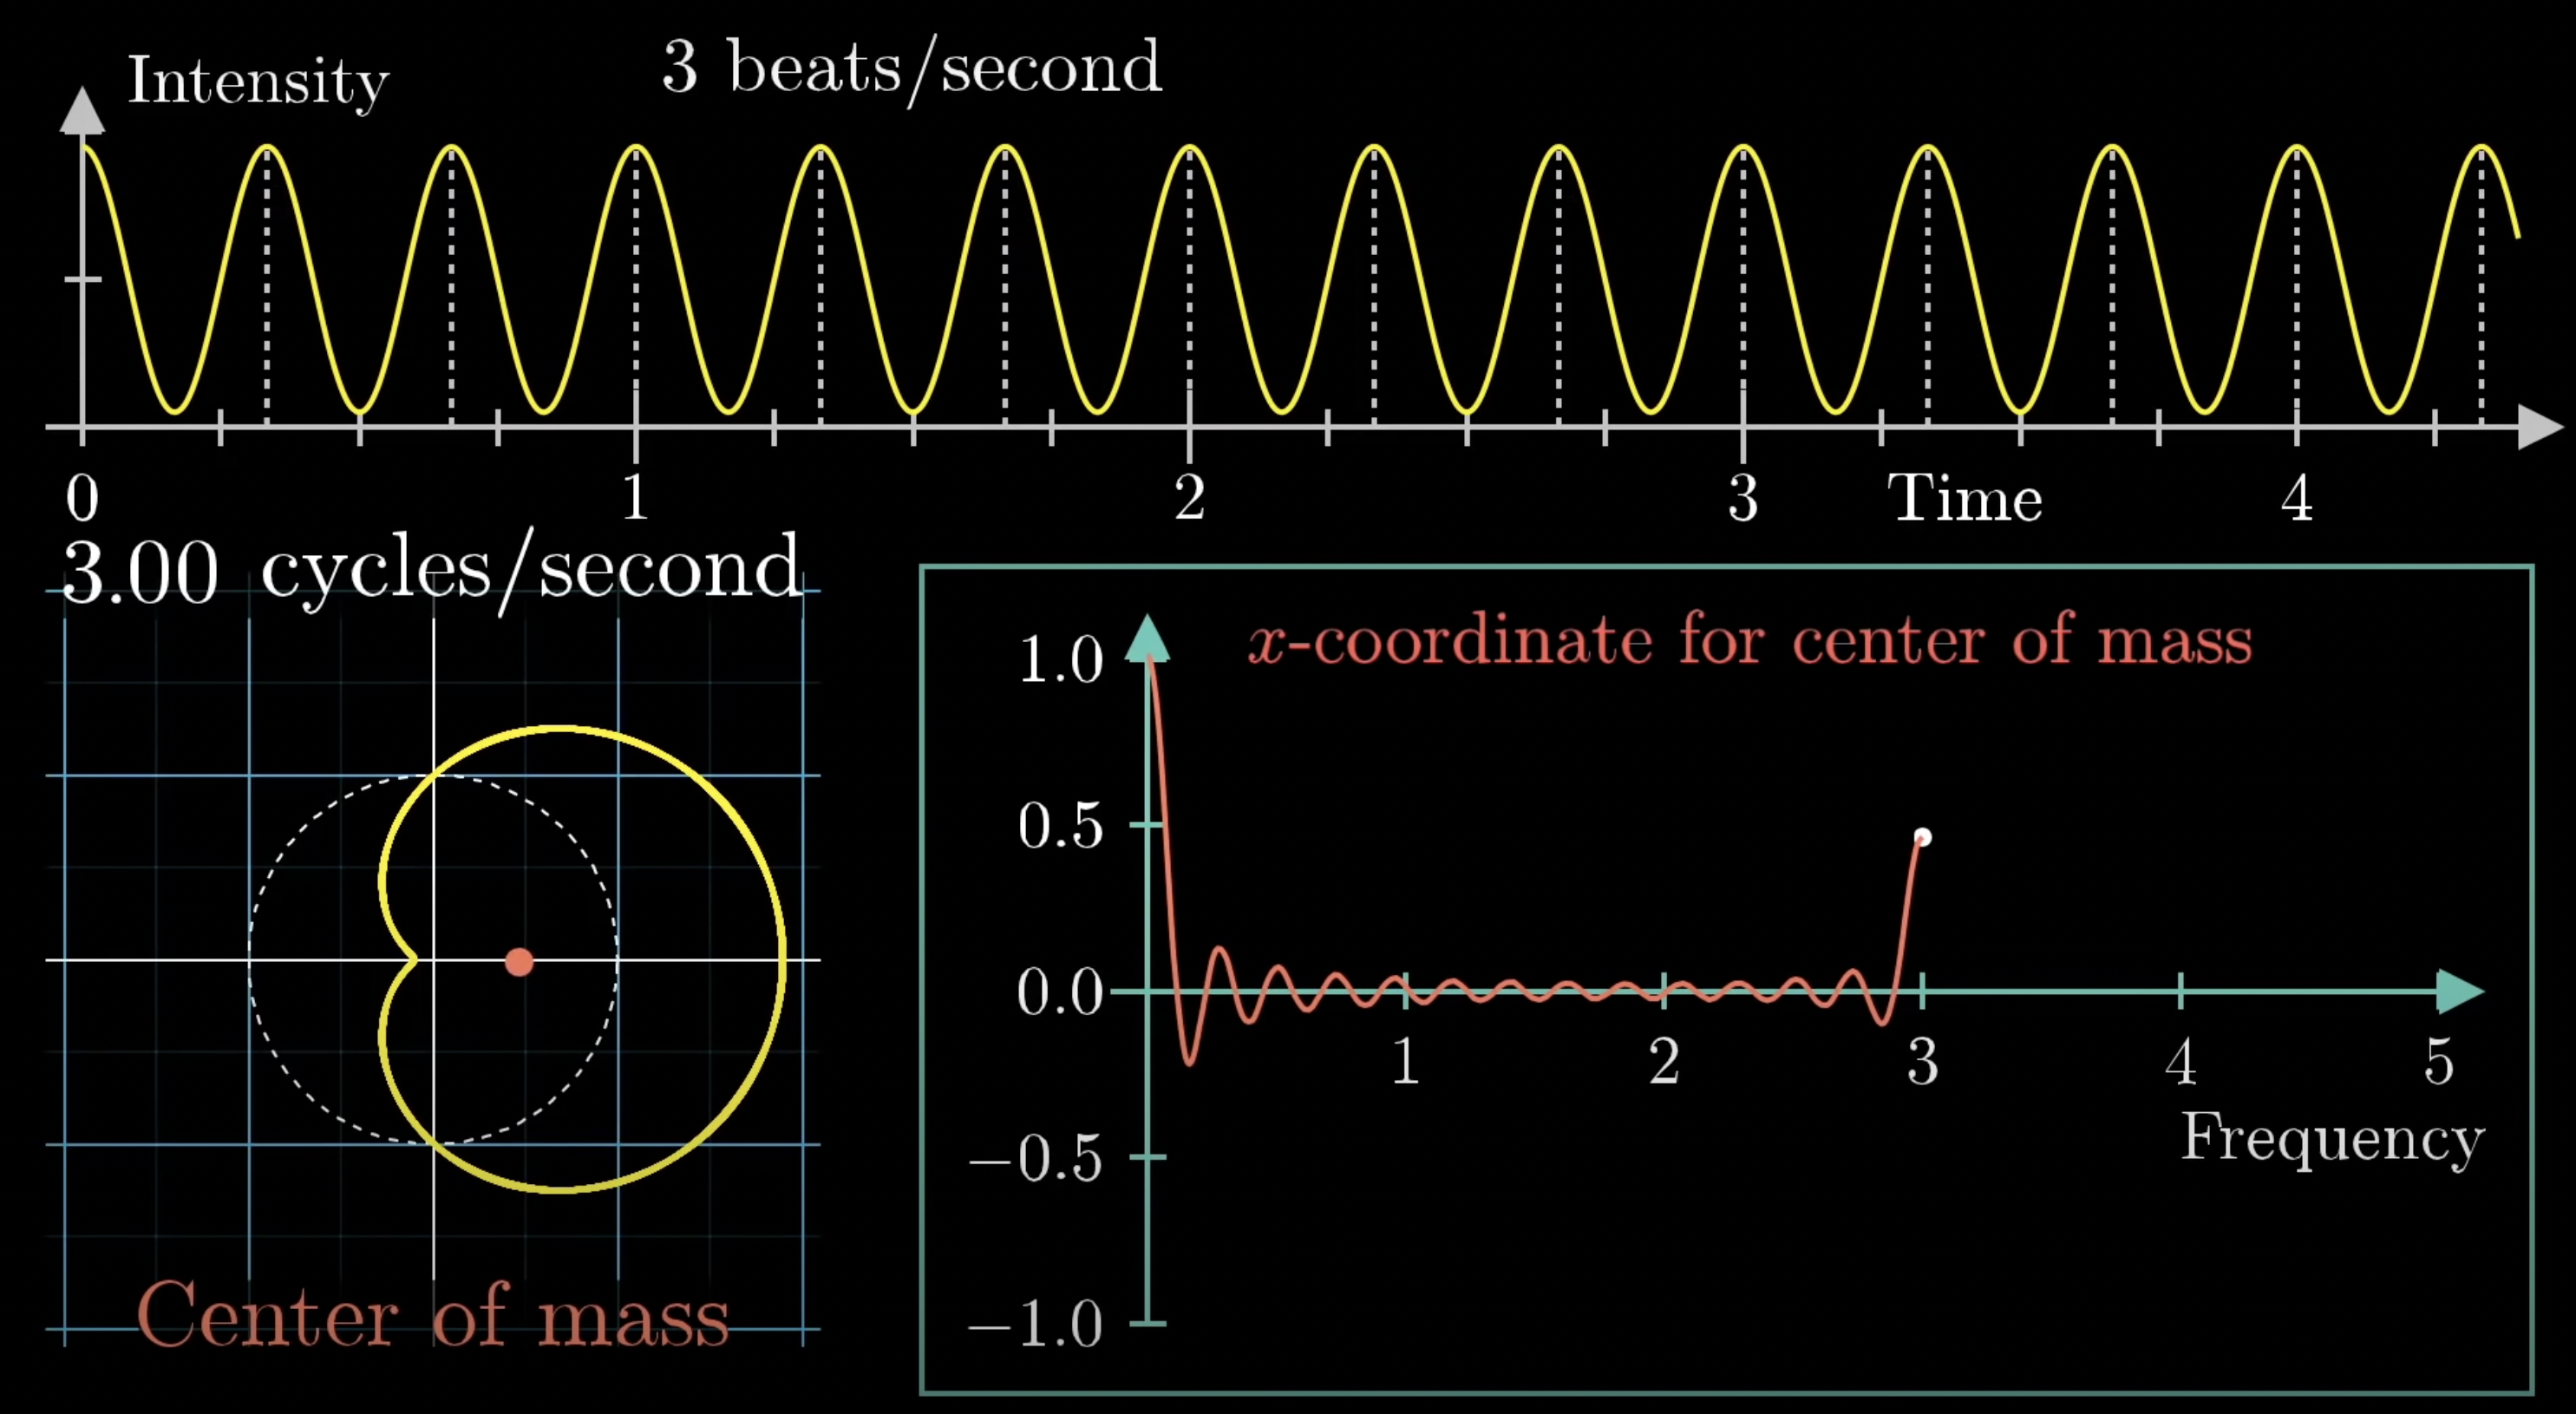
\includegraphics[width=\linewidth]{fft.png}
  \caption[Illustration of how FFT works]{Illustration of how FFT works \citep{3blue1brown_but_2018}}
  \label{fig:fft}
\end{figure}

The process of FFT is represented visually in \autoref{fig:fft}. A given frequency in the timeseries is used to calculate the cycles to extract the originally occurring frequency signal based on the epoch length. As a result, we have per-sample and epoch-based classification of neural data, which can be real-time, real-time with an initial delay to buffer a given epoch (as with FFT), or asynchronous and not real-time, as with sleep phases. Figure 123 visualises the differences between these three stream types.

% TODO create figure for epoch vs per sample incl buffering

\subsubsection{Critical and non-critical}
\label{chapter5-critical-and-non-critical}

The discussion of stream-based events leads us to the aspect of critical and non-critical use cases. In a critical use case such as microsleep detection while driving, we need a synchronous neural stream with low-latency classification of whether the driver is currently awake, asleep or about to fall asleep. In such use cases, the classification needs to be as fast as possible, such as in per-sample classification or epoch-based classification (most likely with buffer), so it is more about how fast the connection between the measurement sensor and the classifier is. In very critical use cases, where e.g. a user's life may depend on it, the classification would need to be done without an active internet connection, so that the classification model runs on the hardware itself and not in the cloud, in order to be able to intervene within milliseconds (e.g. in the form of a loud sound to warn or wake up the driver), as a few moments can make the difference between fatalities.

Not-so-critical applications can fall back on non-offline modes and run classifiers over an active internet connection in the cloud. To reduce latency, edge cloud computing could be introduced, where business logic executed in the cloud is brought geographically closer to the end user via edge locations \citep{nomios_what_nodate}. The aspect of edge-computing is a topic that is not covered in the aspects of a N/CI in this thesis since it was not q requirement to build a critical system at IDUN.

However, the distinction between critical and non-critical streams can be made not only for synchronous streams, as described in the preceding examples, but also for asynchronous streams, particularly in the context of research. In general, research represented by e.g. IDUN's Persona Noel does not necessitate synchronous streams or real-time classifications, but rather the most reliable possible acquisition of neural data from test subjects. The critical aspect in such a use case can also be much higher than, e.g. recording neural data during sleep in consumer-oriented applications. For example, if the device goes offline or the Bluetooth connection is lost, the device must cache the data locally and be able to restore it once the device is back in range or a sufficiently stable internet connection is restored. The author recommends having a fallback system in the form of buffering for each data stream, for example, if neural data becomes corrupted or misordered due to timestamp mismatches in the cloud. Figure 123 illustrates the buffering mechanism.

% TODO create figure for buffering on device and on phone when offline or out of range

\subsubsection{Encryption and opt-in}
\label{chapter5-user-side-opt-in}

Because IDUN develops an unobtrusive library (in the form of an SDK, as detailed in \autoref{appendix4-further-implementation-key-events}) that can be easily implemented in existing software such as web apps or mobile apps, the developers of these apps have actual access to the hardware and initiate the Bluetooth connection between the sensor and the end-user device. IDUN must encrypt the recorded data on the hardware before it reaches the third-party app to protect user privacy and the security of end-user neural data. This is a critical step in preventing third-party providers from collecting extensive data and classifying insights from users that they may not want. In the asynchronous encryption example, IDUN securely decrypts the data in its cloud using the private key. Figure 123 illustrates how the encryption mechanism.

% TODO show figure of how encryption works with private keys etc.

Third-party developers can thus only access data that the user has authorised. The duration of data storage, the type and level of detail of certain classifications of their neural data, and sharing and usage analysis are all opt-in options. Figure 3 depicts how such an opt-in mechanism might appear as a GUI in a third-party mobile app.

% TODO show opt-in mechanism (say that the full version is in the appendix 123)

The fact that unencrypted raw data should never be accessible to third parties poses some technical challenges. To visualise and display the raw time series of IDUN's EEG sensors, e.g. the individual display images would have to be rendered on the server side and streamed to the client as a video stream. Another difficulty is synchronising and organising the rotation of public and private keys, which must be done without interference from third parties. Envelope encryption, as shown in Figure 123, is a tried and true method for this \citep{google_cloud_envelope_nodate}.

% TODO Show figure of envelope encryption \citep{google_cloud_key_nodate}

\subsubsection{Graph data access}
\label{chapter5-graph-data-access}

Aside from the stream-oriented, event-driven nature of a N/CI, the aspect of data storage is critical. It is important to note that, due to the high frequency of the EEG data, it became clear during the implementation phase that storing the neural data in a database is not an efficient method. Storing it as a static file on an object storage system like AWS S3 in a text-based file format like comma-separated values (CSV files seemed more appropriate and scalable. Table 123 shows the data structure of the file that is being stored as a CSV.

% TODO create data structure table

In addition to storing the neural data in the given data structure, it is important to note that other sensor data, such as inertial measurement unit (IMU) data, which is also collected by the IDUN hardware to track the subject's location, rotation, and movement, is also stored alongside and synchronised with the neural data. In addition to the two time-series-based data, EEG and IMU, IDUN collects meta-information such as classified versions of the data, such as eye movement data, which must also be synchronised with the raw data streams. The more classification and post-processing logic that is applied to raw neural data streams, the more metadata must be linked to the original files in a database as figure 123 shows.

% TODO create figure with graph association

A graph database is the most natural way to store this large number of relationships between various stored files (entities). Relationships are treated as first-class citizens in graph databases, and the majority of their value is derived from these relationships. In graph databases, nodes are used to store data entities, while edges are used to store relationships between entities \citep{amazon_web_services_inc_what_nodate}. Due to time limitations the author did not implement a real graph data base but rather has chosen a relation database such as AWS Aurora since the current amount of data relationships is still manageable. To still easily swap the underlying database technology without rewriting a bit portion of the business logic, the author intends to use a object–relational mapping (ORM) tool such as Prisma to treat relational data models as a graph-like schemas \citep{prisma_data_nodate}.

\subsection{Example architecture of a N/CI}
\label{chapter5-example-architecture-of-a-nci}

Based on the key aspects of the N/CI for IDUN's NIP mentioned in the previous subsection the author presents as one of the main results the following cloud architecture in \autoref{fig:example-architecture}.

\begin{figure}[!ht]
  \centering
  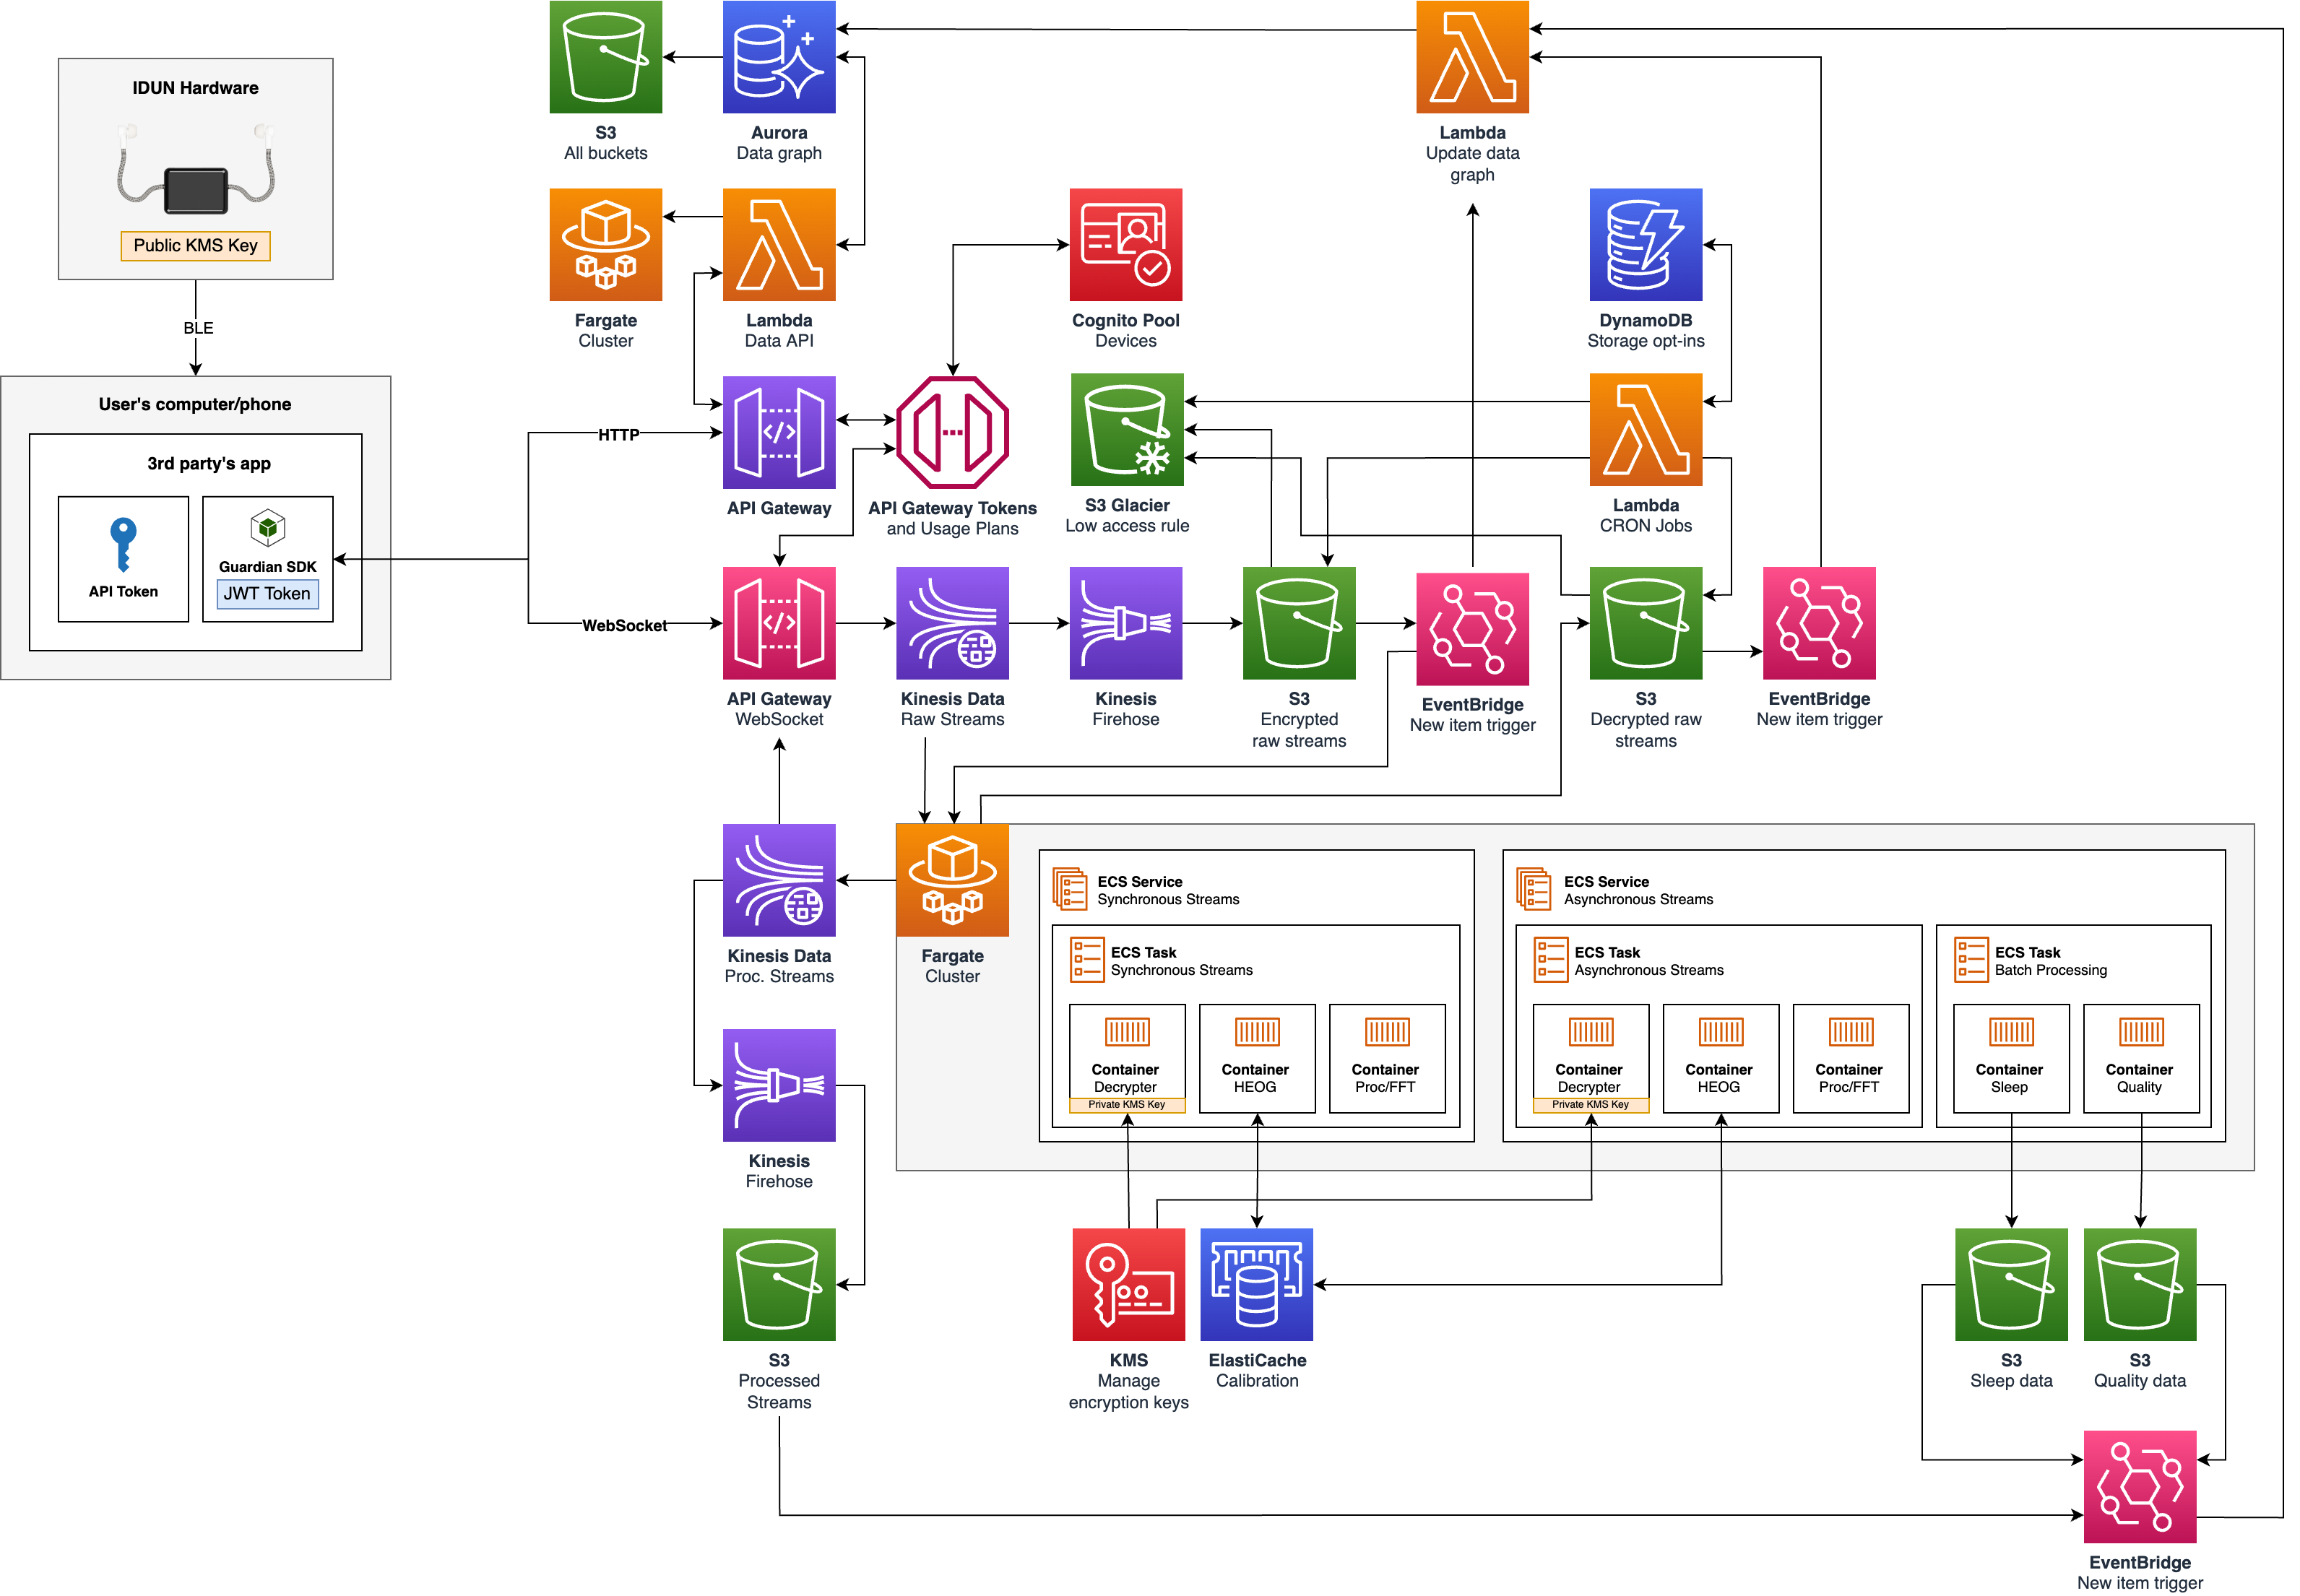
\includegraphics[width=\linewidth]{example-architecture.png}
  \caption{Implementation architecture for IDUN Technologies' N/CI.}
  \label{fig:example-architecture}
\end{figure}

The architecture diagram contains some patterns that have specific reasons. The following list describes the different patterns and sections of the mapped architecture and the associated technical descriptions. It is important to note that some parts are not discussed as they are not part of this work, such as the networking aspect of the cloud setup (e.g. virtual private clouds (VPCs), network address translation services (NATs) and security groups and their traffic rules).

\begin{itemize}
\item \begin{figure}[!ht]
  \centering
  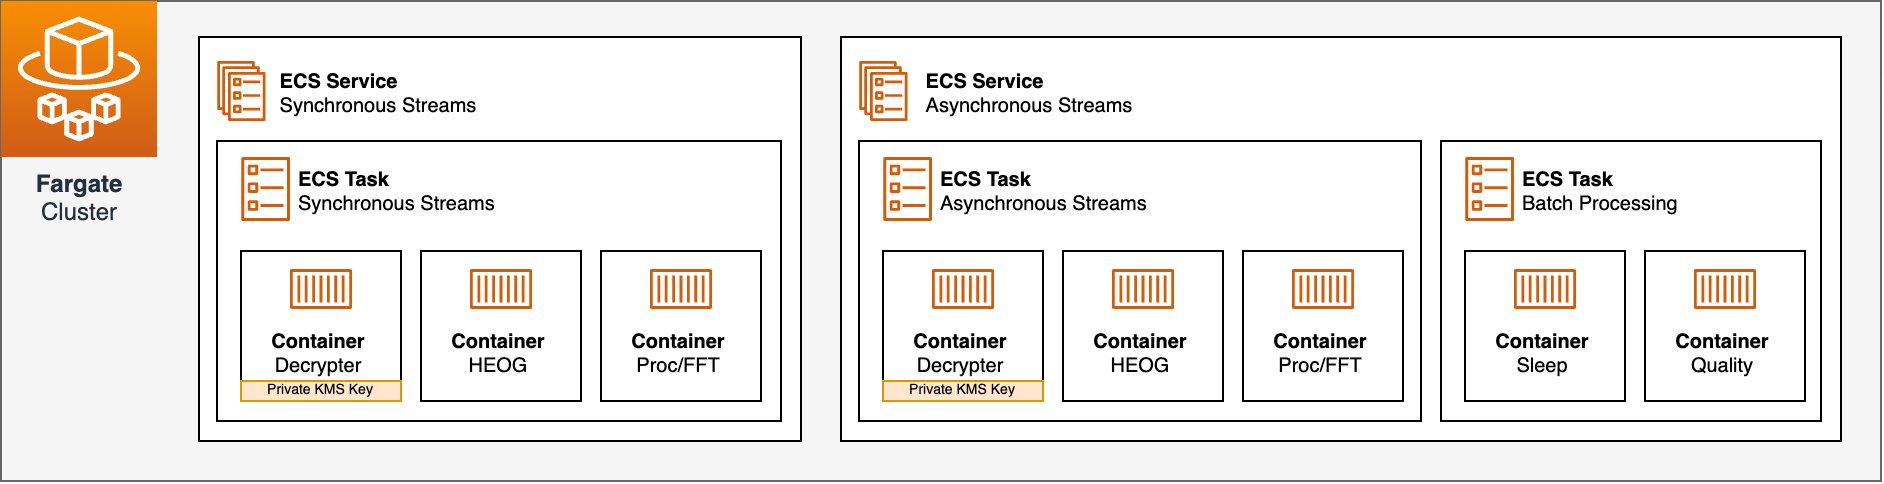
\includegraphics[width=\linewidth]{cluster.png}
  \caption{The Fargate cluster of the example architecture.}
  \label{fig:cluster}
\end{figure}

This is a text for figure 123.

\item  \begin{figure}[!ht]
  \centering
  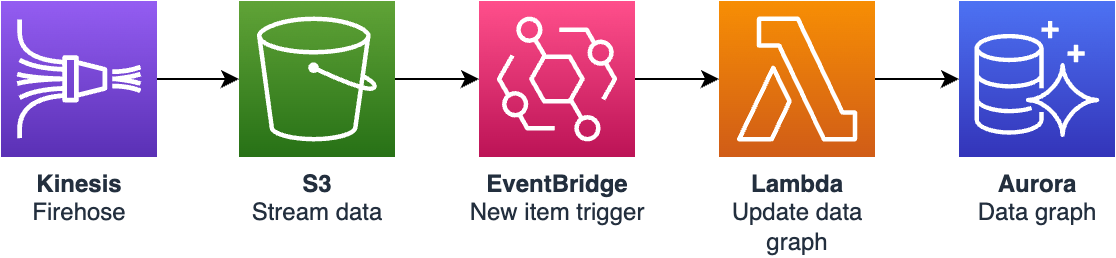
\includegraphics[width=\linewidth]{initial-dataflow.png}
  \caption{The initial data flow.}
  \label{fig:initial-flow}
\end{figure}

This is some more info.

\item  \begin{figure}[!ht]
  \centering
  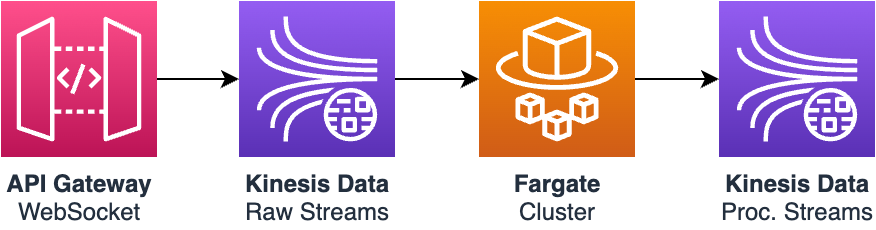
\includegraphics[width=\linewidth]{real-time-dataflow.png}
  \caption{The real-time data flow.}
  \label{fig:realtime-flow}
\end{figure}

Real-time data flow example etc.

\item \begin{figure}[!ht]
  \centering
  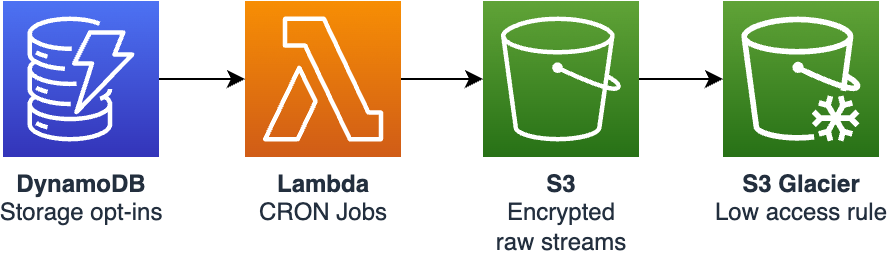
\includegraphics[width=\linewidth]{cron-jobs.png}
  \caption{CRON jobs.}
  \label{fig:cron}
\end{figure}

Cron jobs etc.

\item \begin{figure}[!ht]
  \centering
  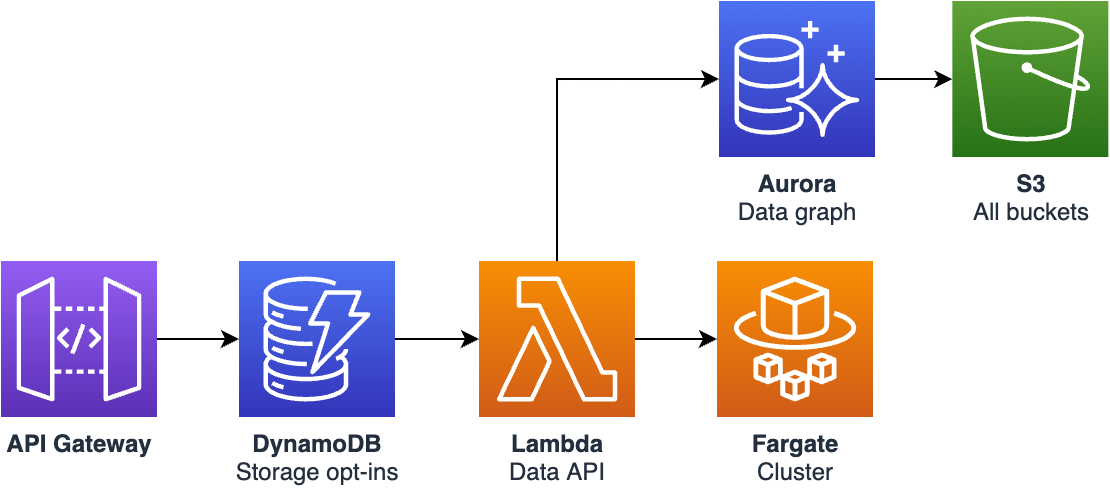
\includegraphics[width=\linewidth]{api-access.png}
  \caption{API access part of the architecture.}
  \label{fig:api-access}
\end{figure}

API access part of the architecture.

\end{itemize}


% TODO insert list

% non-trivial, n-tier system, Services, batch processing and near real time streaming, shared nothing, encrypted, total order broadcast etc. => all insights that were gained for the N/CI and the task to define a N/CI on its own as well + Systems of record and derived data system (p 602 to cite) ==> add some parts to the implementation chapter

\section{Summary}
\label{chapter5-summary}

This section summarises the thesis' outputs and success criteria, as well as a conclusion about the project and its importance. A critical examination and reflection of the author's approach will also be conducted.

% TODO write more

\subsection{Reflection}
\label{chapter5-reflection}

The creation of an example N/CI in the industry as part of IDUN Technologies' NIP was a non-trivial and complex endeavour. There were many moving parts and a lot of uncertainties. Since there is also no other person publicly building a N/CI, or something that would fall into the category of a N/CI, the author could not fall back on experienced engineers who built such as system for a mass-market BCI. The biggest problem as part of this work was the sheer scope of the project as it can be reflected by the length of the thesis. Now in retrospect, it might have been better to set a more clear focus on what the effective deliverable might be, rather than having four objectives and main goals as mentioned in the earlier subsection. The author should also have defined more clear criteria of what the work packages should have been and what would define them as finished, such as in the DoD practise in Scrum.

\subsection{Outlook}
\label{chapter5-outlook}

The author aims to publish certain parts of this thesis in form of a scientific paper. Most interestingly is the part about the definition and motivation behind creating the new discipline in which neural/cloud interfacing resides in. Next to that the author will continue to work at IDUN Technologies to further develop their N/CI and document the upcoming technological challenges.

One big aspect and shift that will arise as soon as IDUN would sell their device to the general public is that the currently proposed architect as e.g. shown in \autoref{chapter5-example-architecture-of-a-nci} is for a localised system, i.e. the cloud data centre is located at one geographical location. As an outlook it might be noteworthy to have a look at a distributed cloud system since scaling around the population around the globe would dictate to create a distributed system to reduce latency and fault tolerance. This aspect could e.g. be done as a master thesis for the author's upcoming career plans.

\subsection{Conclusion}
\label{chapter5-conclusion}

% - We investigated whether depression can be treated by training a positive focus
% - Our findings confirm this
% - Novel perspective on depression
% - More research needed, more treatments that follow this approach should be developed

\nomenclature[fft]{FFT}{Fast Fourier transform}
\nomenclature[csv]{CSV}{Comma-separated values}
\nomenclature[imu]{IMU}{Inertial measurement unit}
\nomenclature[vpc]{VPC}{Virtual private cloud}
\nomenclature[nat]{NAT}{Network address translation}
\nomenclature[orm]{ORM}{Object–relational mapping}